\chapter{\sffamily Distributed state networks}

{\bfseries\sffamily Concept.} To define and develop an archetype simulation environment for distributed state networks. In our classification scheme, this archetype is defined by an arbitrary, bidirectional state partition graph topology and would make sense for simulations of human brain or traffic control networks and power or water grids. We will also discuss the typical ways in which the state of the system (and its various partitions) may only partially be observed in realistic examples, and analyse how best to deal with each situation. For the mathematically-inclined, this chapter will define the mapping of our formalism to distributed state networks. For the programmers, the software which is designed and described in this chapter can be found in the public Git respository here: \href{https://github.com/worldsoop/worldsoop}{https://github.com/worldsoop/worldsoop}.

\section{\sffamily Defining the archetype}

The distributed state network archetype refers to simulation environments whose bidirectional state partition graph topology is completely arbitrary, requiring no particular connectivity structure at all. Each state partition in this archetype typically refers to the same type of real-world node, object or sub-model. Due to the flexibility in topological structure, this archetype is well-suited to `network' models of realistic phenomena. We have illustrated the state partition graph which fits into this category in Fig.~\ref{fig:state-partition-graph-distributed-state-networks}.

\begin{figure}[h]
\centering
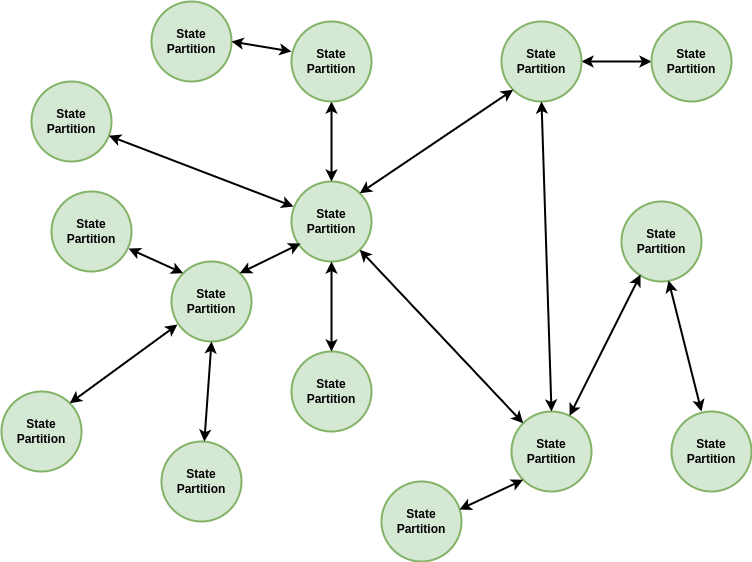
\includegraphics[width=12cm]{images/chapter-8-state-partition-graph.drawio.png}
\caption{State partition graph topology for distributed state network archetypes.}
\label{fig:state-partition-graph-distributed-state-networks}
\end{figure}

Before discussing what kinds of data are typically available to infer states and parameters of environments in this archetype, it will be informative to consider the various real-world problem domains which apply. The particular subset of these domains which seem best suited to this classification include:
%%
\begin{itemize}
\item{Computational models of human brain conditions, e.g., Parkinson's disease~\cite{lu2019application}, epilepsy~\cite{pineau2009treating}, Alzheimer's~\cite{saboo2021reinforcement}, etc., for deep brain stimulation control and other forms of treatment.}
\item{Simulations of complex urban infrastructure networks to target various kinds of optimisation, e.g., traffic signal control~\cite{yau2017survey}, power dispatch~\cite{li2021integrating} and water pipe maintainance~\cite{bukhsh2023maintenance}.}
\end{itemize}
%%